\begin{frame}{Αισθητήρας lidar δισδιάστατων μετρήσεων απόστασης}

  \noindent\makebox[\linewidth][c]{%
  \begin{minipage}{\linewidth}
    \begin{minipage}{0.3\linewidth}
      \begin{figure}
        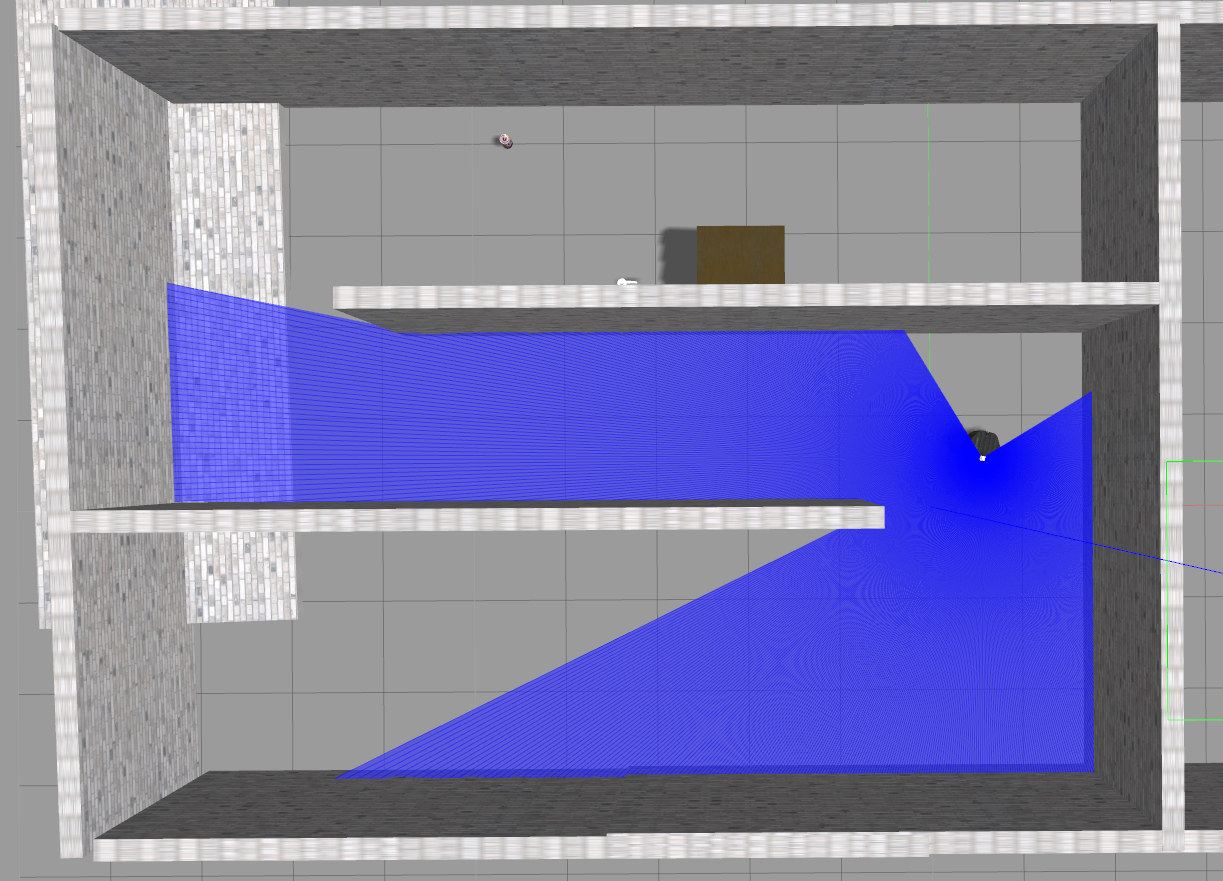
\includegraphics[scale=0.1]{./figures/slides/ch4/gazebo_scan_np.png}
        \caption{\scriptsize Κάτοψη περιβάλλοντος και ακτίνες αισθητήρα}
      \end{figure}
    \end{minipage}
    \hfill
    \begin{minipage}{0.3\linewidth}
      \begin{figure}
        \scalebox{0.8}{% GNUPLOT: LaTeX picture with Postscript
\begingroup
  \makeatletter
  \providecommand\color[2][]{%
    \GenericError{(gnuplot) \space\space\space\@spaces}{%
      Package color not loaded in conjunction with
      terminal option `colourtext'%
    }{See the gnuplot documentation for explanation.%
    }{Either use 'blacktext' in gnuplot or load the package
      color.sty in LaTeX.}%
    \renewcommand\color[2][]{}%
  }%
  \providecommand\includegraphics[2][]{%
    \GenericError{(gnuplot) \space\space\space\@spaces}{%
      Package graphicx or graphics not loaded%
    }{See the gnuplot documentation for explanation.%
    }{The gnuplot epslatex terminal needs graphicx.sty or graphics.sty.}%
    \renewcommand\includegraphics[2][]{}%
  }%
  \providecommand\rotatebox[2]{#2}%
  \@ifundefined{ifGPcolor}{%
    \newif\ifGPcolor
    \GPcolorfalse
  }{}%
  \@ifundefined{ifGPblacktext}{%
    \newif\ifGPblacktext
    \GPblacktexttrue
  }{}%
  % define a \g@addto@macro without @ in the name:
  \let\gplgaddtomacro\g@addto@macro
  % define empty templates for all commands taking text:
  \gdef\gplbacktext{}%
  \gdef\gplfronttext{}%
  \makeatother
  \ifGPblacktext
    % no textcolor at all
    \def\colorrgb#1{}%
    \def\colorgray#1{}%
  \else
    % gray or color?
    \ifGPcolor
      \def\colorrgb#1{\color[rgb]{#1}}%
      \def\colorgray#1{\color[gray]{#1}}%
      \expandafter\def\csname LTw\endcsname{\color{white}}%
      \expandafter\def\csname LTb\endcsname{\color{black}}%
      \expandafter\def\csname LTa\endcsname{\color{black}}%
      \expandafter\def\csname LT0\endcsname{\color[rgb]{1,0,0}}%
      \expandafter\def\csname LT1\endcsname{\color[rgb]{0,1,0}}%
      \expandafter\def\csname LT2\endcsname{\color[rgb]{0,0,1}}%
      \expandafter\def\csname LT3\endcsname{\color[rgb]{1,0,1}}%
      \expandafter\def\csname LT4\endcsname{\color[rgb]{0,1,1}}%
      \expandafter\def\csname LT5\endcsname{\color[rgb]{1,1,0}}%
      \expandafter\def\csname LT6\endcsname{\color[rgb]{0,0,0}}%
      \expandafter\def\csname LT7\endcsname{\color[rgb]{1,0.3,0}}%
      \expandafter\def\csname LT8\endcsname{\color[rgb]{0.5,0.5,0.5}}%
    \else
      % gray
      \def\colorrgb#1{\color{black}}%
      \def\colorgray#1{\color[gray]{#1}}%
      \expandafter\def\csname LTw\endcsname{\color{white}}%
      \expandafter\def\csname LTb\endcsname{\color{black}}%
      \expandafter\def\csname LTa\endcsname{\color{black}}%
      \expandafter\def\csname LT0\endcsname{\color{black}}%
      \expandafter\def\csname LT1\endcsname{\color{black}}%
      \expandafter\def\csname LT2\endcsname{\color{black}}%
      \expandafter\def\csname LT3\endcsname{\color{black}}%
      \expandafter\def\csname LT4\endcsname{\color{black}}%
      \expandafter\def\csname LT5\endcsname{\color{black}}%
      \expandafter\def\csname LT6\endcsname{\color{black}}%
      \expandafter\def\csname LT7\endcsname{\color{black}}%
      \expandafter\def\csname LT8\endcsname{\color{black}}%
    \fi
  \fi
    \setlength{\unitlength}{0.0500bp}%
    \ifx\gptboxheight\undefined%
      \newlength{\gptboxheight}%
      \newlength{\gptboxwidth}%
      \newsavebox{\gptboxtext}%
    \fi%
    \setlength{\fboxrule}{0.5pt}%
    \setlength{\fboxsep}{1pt}%
\begin{picture}(3000.00,3000.00)%
    \gplgaddtomacro\gplbacktext{%
    }%
    \gplgaddtomacro\gplfronttext{%
      \colorrgb{0.00,0.00,0.00}%
      \put(1595,2153){\makebox(0,0)[l]{\strut{}\scriptsize \texttt{5}}}%
      \put(1723,2697){\makebox(0,0)[l]{\strut{}\scriptsize \texttt{10}}}%
      \put(2682,1500){\makebox(0,0)   {\strut{}\scriptsize $0^\circ$}}%
      \put(2633,2106){\makebox(0,0)   {\strut{}\scriptsize $+30^\circ$}}%
      \put(2224,2550){\makebox(0,0)   {\strut{}\scriptsize $+60^\circ$}}%
      \put(1467,2713){\makebox(0,0)   {\strut{}\scriptsize $+90^\circ$}}%
      \put(809,2550){\makebox(0,0)    {\strut{}\scriptsize $+120^\circ$}}%
      \put(300,2106){\makebox(0,0)    {\strut{}\scriptsize $+150^\circ$}}%
      \put(251,1500){\makebox(0,0)    {\strut{}\scriptsize $180^\circ$}}%
      \put(300,893){\makebox(0,0)     {\strut{}\scriptsize $-150^\circ$}}%
      \put(709,449){\makebox(0,0)     {\strut{}\scriptsize $-120^\circ$}}%
      \put(1466,286){\makebox(0,0)    {\strut{}\scriptsize $-90^\circ$}}%
      \put(2124,449){\makebox(0,0)    {\strut{}\scriptsize $-60^\circ$}}%
      \put(2533,893){\makebox(0,0)    {\strut{}\scriptsize $-30^\circ$}}%
    }%
    \gplbacktext
    \put(0,0){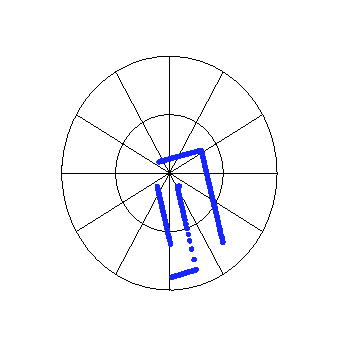
\includegraphics{./figures/slides/ch4/gazebo_scan_np.eps}}%
    \gplfronttext
  \end{picture}%
\endgroup
}
        \caption{\scriptsize Η σάρωση στο σύστημα αναφοράς αισθητήρα}
      \end{figure}
    \end{minipage}
    \hfill
    \begin{minipage}{0.3\linewidth}
      \begin{figure}\hspace{-1cm}
        \scalebox{0.5}{\definecolor{b}{RGB}{22 38 252}
\begin{tikzpicture}

  \coordinate (O) at (0,0);
  \node (O_n) at (0.2,-0.2) {$O$};
  \node (x_plus) at (3.5,0) {$x$};
  \node (y_plus) at (0,3) {$y$};
  \coordinate (x_minus) at (-2,0);
  \coordinate (y_minus) at (0,-2.5);
  \coordinate (first_ray) at (-2*0.70711, -2*0.70711);
  \coordinate (first_ray_far) at (-2.5*0.70711, -2.5*0.70711);
  \node (ray_0) at (-3.0*0.70711, -3.0*0.70711){ακτίνα $0$};
  \coordinate (last_ray) at (-2*0.70711, 2*0.70711);
  \coordinate (last_ray_far) at (-2.5*0.70711, 2.5*0.70711);
  \node (ray_N) at (-3.0*0.70711, 3.0*0.70711){ακτίνα $N_s$$-$$1$};
  \node (l) at (-1.0,0.2){$\scriptstyle{2\pi-\lambda}$};
  \coordinate(n_c) at (3.0,1.117);
  \node[right] (n_n) at (1.8,1.5){ακτίνα $n$: $\textcolor{b}{d_n = \mathcal{S}[-\dfrac{\lambda}{2} + \dfrac{\lambda n}{N_s}]}$};
  \draw [fill] (n_c) circle [radius=0.05];
  \draw [fill] (O) circle [radius=0.05];
  \node[above] (dn) at (1.0,0.35){$d_n$};

  % draw axes
  \draw [->] (x_minus) -- (x_plus);
  \draw [->] (y_minus) -- (y_plus);
  \draw [dashed] (O) -- (last_ray_far);
  \draw [dashed] (O) -- (first_ray_far);
  \draw [->] (O) -- (n_c);

  % draw laser arc
  \draw [black, thick, dotted] (first_ray) arc[start angle=-135, end angle=135,radius=2];

  % draw 2π - λ arc
  \pic [draw,  angle radius=5mm, angle eccentricity=1.4] {angle = last_ray--O--first_ray};

  % draw n angle arc
  \pic [draw, ->, angle radius=17mm, angle eccentricity=1.4] {angle = x_plus--O--n_c};
  \node (angle_n) at (2.6,0.44){${\scriptstyle-\dfrac{\scriptstyle\lambda}{\scriptstyle 2} + \dfrac{\scriptstyle \lambda n}{\scriptstyle N_s}}$};

\end{tikzpicture}
}
        \caption{\scriptsize Τοπικό σύστημα αναφοράς αισθητήρα}
      \end{figure}
    \end{minipage}

  \end{minipage}
  }

  \definecolor{b}{RGB}{22 38 252}
  Σάρωση $\mathcal{S} : \Theta \rightarrow \textcolor{b}{\mathbb{R}_{\geq 0}}$, όπου
  \begin{align}
    \Theta &= \{\theta_n \in [-\frac{\lambda}{2}, +\frac{\lambda}{2}) : \theta_n = -\frac{\lambda}{2} + \lambda \frac{n}{N_s}, n = 0,1,\dots, N_s-1\}, \text{ όπου}  \nonumber\\
    \lambda&: \text{Γωνιακό εύρος όρασης} \text{ και } N_s: \text{αριθμός εκπεμπόμενων ακτίνων}\nonumber
  \end{align}


\end{frame}
